\documentclass[11pt,a4paper]{scrartcl}
\usepackage[english]{babel}
\usepackage[utf8]{inputenc}
\usepackage[T1]{fontenc}
\usepackage{lmodern}
\usepackage{amsmath}
\usepackage{amsthm}
\usepackage{amssymb}
\usepackage{enumitem}
\usepackage[hidelinks]{hyperref}
\usepackage{graphicx}
\usepackage{listings}
\usepackage{placeins}

\graphicspath{{./Figures/}}

\newtheorem*{theorem}{Theorem}
\theoremstyle{definition}
\newtheorem*{definition}{Definition}

\setlength{\parindent}{0cm}
\title{Machine Learning Final Project}
\subtitle{Seq2seq Model}
\author{Siyang Sun, Kevin Xie}
\date{\today}

\begin{document}
\begin{titlepage}
	\centering
	{\Huge\bfseries Insights into Seq2seq Models for Text Correction\par}
	\vspace{7cm}
	{\LARGE\itshape Kevin Xie (UID: 304402775)\par}
	\vspace{.9em}
	{\LARGE\itshape Siyang Sun (UID: 504400191)\par}
	\vspace{.9em}


	\vfill

\end{titlepage}
\tableofcontents

\section{Introduction}
One field of application for differential equations is population dynamics - a biological discipline that analyzes the long-term behavior of populations of different species in an ecological system. This project deals with two-species models based on the so-called Lotka-Volterra equations. Let $N_1$ and $N_2$ denote the population of two distinct species. Assuming that they interact with each other directly, there are three different kinds of relationships between $N_1$ and $N_2$ that can occur \cite{Murray}:

\begin{itemize}
	\item{The two species are in a \textbf{predator-prey} relationship, in which $N_1$ is threatened by the presence of $N_2$, but $N_2$ is enhanced by $N_1$.}
	\item{The two species are said to be in \textbf{competition} if both species affect each other negatively, i.e. the existence of $N_1$ is a threat to $N_2$ and vice versa.}
	\item{\textbf{Mutualism} is a relationship in which the two species affect each other positively, i.e. the existence of $N_1$ benefits $N_2$ and vise versa.}
\end{itemize}

\section{Seq2seq Model}
Let $N_1$ denote the population of the prey and $N_2$ the population of the predator, then the relationship between the two species can be described by the simple model \cite{Haberman}:

\begin{equation} \label{eq1}
	\frac{dN_1}{dt}=N_1(a-bN_1-cN_2),
\end{equation}

\begin{equation} \label{eq2}
	\frac{dN_2}{dt}=N_2(dN_1-e)
\end{equation}

with constants $a,c,d,e \in \mathbb{R}_{>0}$ and $b \in \mathbb{R}_{\geqslant 0}$.
\newline

Before analyzing this system of differential equations mathematically, let us try to get a better understanding of this model.

Suppose that $N_2 \equiv 0$, then equation \eqref{eq1} reduces to the one-species model:

\begin{equation} \label{eq3}
	\frac{dN_1}{dt}=N_1(a-bN_1). 
\end{equation}

In the absence of predators, if the initial population $N_0^{1}:=N_1(0)$ is less than $\frac{a}{b}$, the population of prey increases. Similarly, if the initial population $N_0^{1}$ is greater than $\frac{a}{b}$, the population of prey decreases. In either case, the growth or decay limits at the equilibrium population $\frac{a}{b}$, which is, however, never reached, except for the constant solution $N_1 \equiv \frac{a}{b}$. In fact, equation \eqref{eq3} is well-known as the \textit{logistic equation}. Since the focus of this project lies on two-species systems, further analysis of equation \eqref{eq3} is left to the reader. Suppose that $N_1 \equiv 0$, then equation \eqref{eq2} reduces to:

\begin{equation} \label{eq4}
	\frac{dN_2}{dt}=-eN_2.
\end{equation}

This means that without prey the population of predators decreases at all times. All the previous aspects reflect what might be expected from a predator-prey relationship. Nevertheless, the stated model imposes some implicit assumptions that do not necessarily apply to reality, but simplify the complex and interwoven influencing factors within an ecological system. For example, our model is limited on the interaction of precisely two species, so predators feed on only one prey, and other possible food sources are not considered. For the validity of this model, we must also assume the absence of migration and unforeseen catastrophes. 

\subsection{Equilibrium Populations and Stability}
The fixed points of models in population dynamics are also called equilibrium populations, and correspond to constant solutions.
As a reminder the definition is stated below.
\begin{definition}{\textbf{\textit{Equilibrium Populations}}}
\newline
Let $\frac{dN_1}{dt}=f(N_1, N_2)$ and $\frac{dN_2}{dt}=g(N_1, N_2)$. Equilibrium populations are all points $(N_1^{*}, N_2^{*}) \in \mathbb{R}^2$ with $N_1^{*}, N_2^{*} \geqslant 0$ such that $f(N_1^{*},N_2^{*})=0$ and $g(N_1^{*},N_2^{*})=0$ \cite{main}. 
\end{definition}
Notice that equilibrium populations are restricted to $\mathbb{R}_{\geqslant 0}^2$ because of the biological background of the models.

\subsubsection{Special Case}
First, let us consider the special case of our model where $b=0$. Then equation \eqref{eq1} becomes:

\begin{equation} \label{eq5}
	\frac{dN_1}{dt}=N_1(a-cN_2).
\end{equation}
	
In this even simpler predator-prey model the population growth of the prey in absence of predators is unbounded from above. There are exactly two equilibrium populations, which are $\alpha=(0,0)$ and $\beta=(\frac{e}{d}, \frac{a}{c})$. To linearize the system around the equilibrium populations we define the function $F(N_1, N_2)=(N_1(a-cN_2), N_2(dN_1-e))$, then we get the Jacobian matrix:

\begin{center}
$DF(N_1, N_2)=\begin{pmatrix}
	\frac{df_1(N_1, N_2)}{dN_1} & \frac{df_1(N_1, N_2)}{dN_2} \\
	\frac{df_2(N_1, N_2)}{dN_1} & \frac{df_2(N_1, N_2)}{dN_2}
\end{pmatrix}
=\begin{pmatrix}
	a-cN_2 & -cN_1 \\
	dN_2 & dN_1-e
\end{pmatrix}$.
\end{center}

Since $det(DF(\alpha))=-ae<0$, the origin is a saddle and unstable. The equilibrium population $\beta$ is more interesting. It is $det(DF(\beta))=ae>0$, $tr(DF(\beta))=0$ and $tr(DF(\beta))^2-4det(DF(\beta))=-4ae<0$, so $\beta$ is called a center. There are various examples showing that a linearized center might differ from a center in a linear system. Hence, a natural question is how solutions of the simplified model behave in a close neighborhood of $\beta$. In this case, the following theorem leads us to the answer.

\begin{theorem}
	Consider the nonlinear system $\dot{\chi}=\vec{f}(\chi)$ where $\vec{f}$ is continuously differentiable. Suppose there is a conserved quantity $E(\chi)$, and that $\chi^{*}$ is an isolated fixed point. If $\chi^{*}$ is a local minimum or maximum of E, then all trajectories sufficiently close to $\chi^{*}$ are closed.
\end{theorem}

Note that $F$ as defined above is continuously differentiable, and $\beta$ is an isolated fixed point. Assume that $N_1$ and 
$N_2$ are always non-zero, then equations \eqref{eq5} and \eqref{eq2} can be rewritten as:

\begin{equation} \label{eq6}
	(dN_1-e)\frac{\dot{N_1}}{N_1}=(a-cN_2)(dN_1-e),
\end{equation}

\begin{equation} \label{eq7}
	(a-cN_2)\frac{\dot{N_2}}{N_2}=(dN_1-e)(a-cN_2).
\end{equation}

Subtracting equation \eqref{eq7} from \eqref{eq6} yields:

\begin{equation} \label{eq8}
	(a-cN_2)\frac{\dot{N_2}}{N_2}-(dN_1-e)\frac{\dot{N_1}}{N_1}=0.
\end{equation}

Observe that the function $E(N_1, N_2)=elog(N_1)+alog(N_2)-dN_1-cN_2$ is a conserved quantity, because differentiation with respect to $t$ results in equation \eqref{eq8}. In particular, we have $\frac{dE}{dt}(\beta)=0$. The Hessian matrix of E is:

\begin{center}
$D^2E(N_1,N_2)=\begin{pmatrix}
	-\frac{e}{N_1^{2}} & 0 \\
	0 & -\frac{a}{N_2^{2}}
\end{pmatrix}$.
\end{center}

Obviously, the matrix $D^2E(\beta)$ is negative definite, so $\beta$ is a local maximum of E. Therefore, by the theorem, $\beta$ behaves like a center, i.e. trajectories in a close neighborhood of $\beta$ are closed, and is Lyapunov stable.

\subsubsection{General Case}
In the case $b>0$ there are exactly three equilibrium populations, which are $\alpha=(0,0)$, $\beta=(\frac{e}{d},\frac{ad-be}{cd})$ and $\gamma=(\frac{a}{b},0)$. Again, we want to linearize the system around the equilibrium populations and define the function
$F(N_1, N_2)=(N_1(a-bN_1-cN_2), N_2(dN_1-e))$ whose Jacobian matrix is:

\begin{center}
$DF(N_1, N_2)=\begin{pmatrix}
	a-2bN_1-cN_2 & -cN_1 \\
	dN_2 & dN_1-e
\end{pmatrix}$.
\end{center}

Similar to the special case, the equilibrium population $\alpha$ is uninteresting. The same computation shows that $\alpha$ remains a saddle, and thus is unstable. Consider the fixed point $\beta$. Since we look at the system of differential equations from the standpoint of population dynamics, we can restrict ourselves to the situation when $ad \geqslant be$, i.e. when $\beta$ lies in the first quadrant of the phase plane. It is:

\begin{center}
$B=DF(\beta)=\begin{pmatrix}
	-\frac{be}{d} & -\frac{ce}{d} \\
	\frac{ad-be}{c} & 0
\end{pmatrix}$,
\end{center}

so $det(B)=\frac{e}{d}(ad-be)\geqslant 0$ and $tr(B)=-\frac{be}{d}<0$. Let $z(B):=tr(B)^2-4det(B)$. There are two cases to differentiate. 
If $ad=be$, then $det(B)=0$ and $z(B)>0$. Hence, linearization around $\beta$ leads to the borderline case of non-isolated fixed points for which correctness is not guaranteed. 
If $ad>be$, then $det(B)>0$ and $z(B)=\frac{e}{d}(\frac{b^2e}{d}-4(ad-be))$. A simple computation shows that 
$\frac{b^2e}{d}-4(ad-be)=0$ if and only if $b=-2d \pm 2d\sqrt{1+\frac{a}{e}}$. Let $I \subset \mathbb{R}$ be the interval 
$I=(0,b_0)$ where $b_0=-2d+2d\sqrt{1+\frac{a}{e}}$. We have $z(B)<0$ if $b \in I$. Hence, in this case $\beta$ is locally a stable spiral. For $b>b_0$, it is $z(B)>0$, and thus $\beta$ is locally a stable node. Linearization leads to the marginal case of stable stars or degenerates if $b=b_0$ for which validity is again questionable.
\newline

Finally, let us linearize the system around $\gamma$. We obtain the matrix:

\begin{center}
$C=DF(\gamma)=\begin{pmatrix}
	-a & -\frac{ac}{b} \\
	0 & \frac{ad}{b}-e
\end{pmatrix}$,
\end{center}

so $det(C)=a(e-\frac{ad}{b})$ and $tr(C)=-a+\frac{ad}{b}-e$. This time there are three cases to distinguish, which are $be<ad$, $be=ad$, and $be>ad$. In the first case, the fixed point $\gamma$ is locally a saddle, because $be<ad$ implies $det(C)<0$. In the second case, we obtain $det(C)=0$ and $tr(C)=-a<0$ leading to the borderline case of non-isolated fixed points. As mentioned before, correctness is not ensured for this result. For $be>ad$ it can be shown that $tr(C)<-a<0$ and $tr(C)^2-4det(C)>0$. In this case $\gamma$ is locally a stable node.

\subsection{Phase Plane Analysis}
Let us complete the information gained by linearization with the analysis of the phase plane. 

\begin{figure}[h]
	\centering
	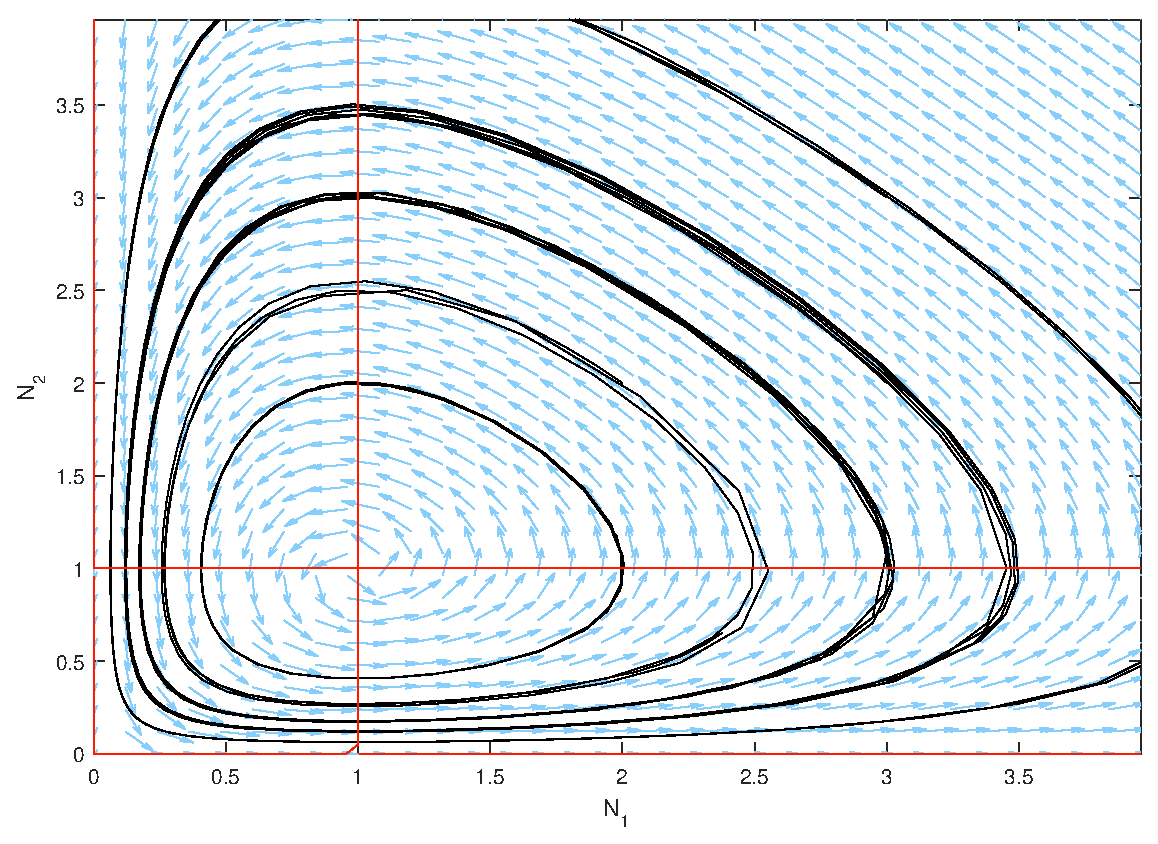
\includegraphics[scale=0.72]{nCenter.eps}
	\caption{Predator-prey model with $a=c=d=e=1$ and $b=0$}
	\label{Center}
\end{figure}
\FloatBarrier

\begin{definition}{\textbf{\textit{Nullclines}}}
\newline
Nullclines are zero level sets of the functions $f=\frac{dN_1}{dt}$ or $g=\frac{dN_2}{dt}$ \cite{main}.
\end{definition}

A vector field for the special case $b=0$ is depicted in figure \ref{Center}. The red lines correspond to the nullclines of the system, which are generally defined by $N_1(1-N_2)=0$ and $N_2(N_1-1)=0$, and the black lines to trajectories of solutions. As predicted by linearization and the stated theorem, the non-trivial equilibrium population at $(1,1)$ is a center. Ecologically, this means the the long-term behavior of the populations $N_1$ and $N_2$ is periodic. Assume that a solution $(N_1,N_2)$ is not constant; then, as the population of prey increases the population of predators rises too. However, at a certain number of predators the population growth of prey becomes negative. After a while, this leads to a shortage of food for the predators resulting in a decreasing population. As a consequence, the prey's population can recover to the starting point, and the cycle repeats. Since we only focus on the first quadrant, it is not obvious by just looking at the phase plane that the origin is locally a saddle. However, the fact that the origin is unstable is more important and can be observed. Note that the constant solution $(0,0)$ reflects the situation in which both species are extinct. The corresponding equilibrium population is always a saddle. Thus, it will not be considered in detail again for the following cases. 
\newline

In the general case where $b>0$, the nullclines are generally given by the two equations $N_1(a-bN_1-cN_2)=0$ and $N_2(dN_1-e)=0$. As before we divide the analysis into the three cases $be<ad$, $be=ad$, and $be>ad$. 

\begin{figure}[h]
	\centering
	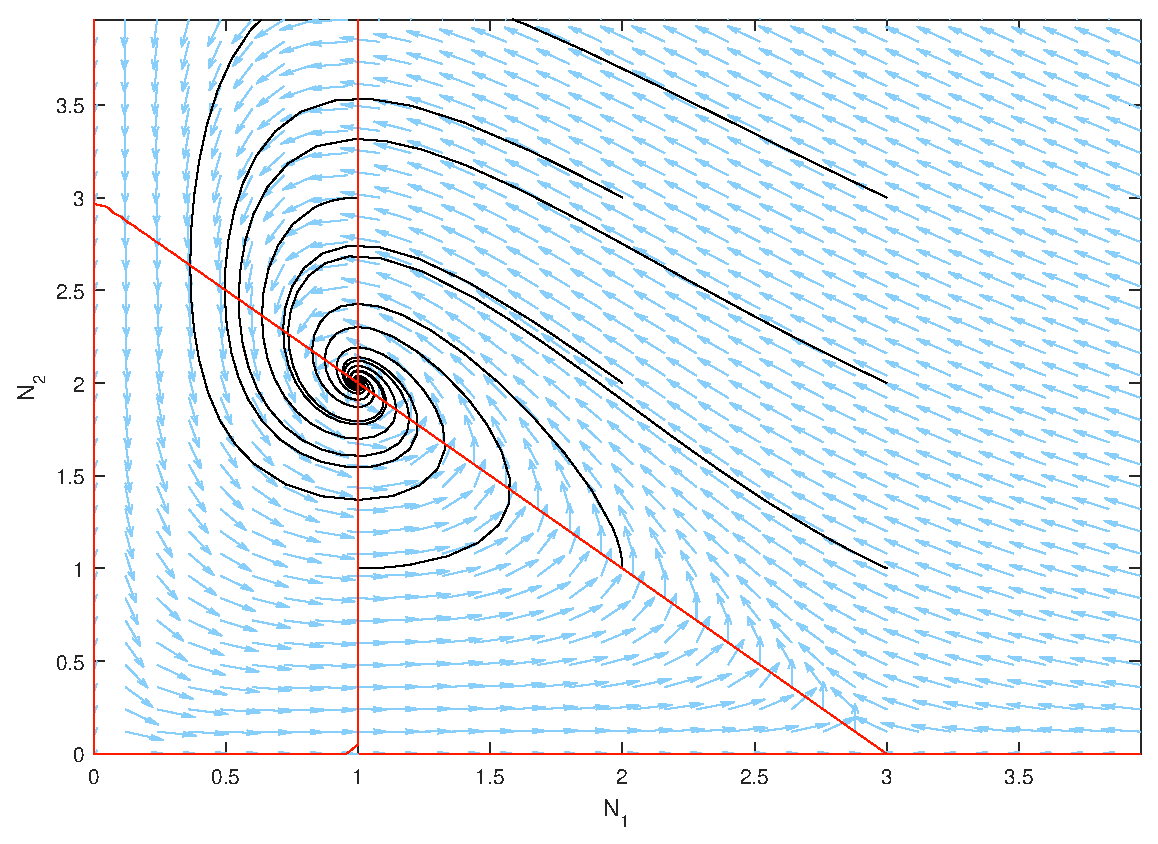
\includegraphics[scale=0.72]{nBeta_StableSpiral.eps}
	\caption{Predator-prey model with $a=3$ and $b=c=d=e=1$}
	\label{fig2}
\end{figure}
\FloatBarrier

First, let us analyze the case $be<ad$. In Figure \ref{fig2}, the equilibrium populations are $\alpha=(0,0)$, $\beta=(1,2)$ and $\gamma=(3,0)$. We see that $\beta$ is a stable spiral, which agrees with the computations before. Suppose that a solution $(N_1,N_2)$ is non-constant; then the long-term development of the populations is no longer periodic. The populations of both species converge to an equilibrium population. If $N_1 \neq 0$ and $N_2 \neq 0$, then the populations approach $\beta$ as $t \rightarrow \infty$. In the absence of predators, when $N_1 \neq 0$ and $N_2 \equiv 0$, the solution converges to $\gamma$ as $t \rightarrow \infty$. This is because we imposed logistic growth for the prey. However, if $N_1 \equiv 0$ and $N_2 \neq 0$, then the population of predators decreases to $\alpha$, since there is no food available. Hence, the first quadrant (excluding the axes) is called \textit{basin of attraction} around $\beta$. The definition is as follows:

\begin{definition}{\textbf{\textit{Basin of Attraction}}}
\newline
A basin of attraction is a set of initial conditions $N_0$ such that N(t) $\rightarrow N^*$ as t $\rightarrow \infty$, where N(t) is a solution trajectory and N* is an attracting fixed point \cite{main}.
\end{definition}

Small deviations in the coefficients of the predator-prey model can lead to significant changes in the qualitative behavior of solution trajectories. Consider Figure \ref{fig3} as an example. For the chosen coefficients the phase portrait deviate more and more from the special case. We have the equilibrium populations $\alpha=(0,0)$, $\beta=(1,2)$ and $\gamma=(1.2,0)$, where this time $\beta$ is (locally) a stable node. If $N_1 \neq 0$ and $N_2 \neq 0$, then both populations converge to $\beta$ as $t \rightarrow \infty$. Thus, the whole first quadrant excluding the axes is a basin of attraction around $\beta$. The behavior of trajectories on the axes are the same as before. The only difference is the position of $\gamma$. Figure \ref{fig4} depicts the phase portrait of the marginal case. The qualitative behavior of the trajectories is identical to the previous case, so that we can speculate that $\beta$ is locally also a stable node in this case.  Note that $\gamma$ is always a saddle for $be<ad$.\newline

\begin{figure}[h]
	\centering
	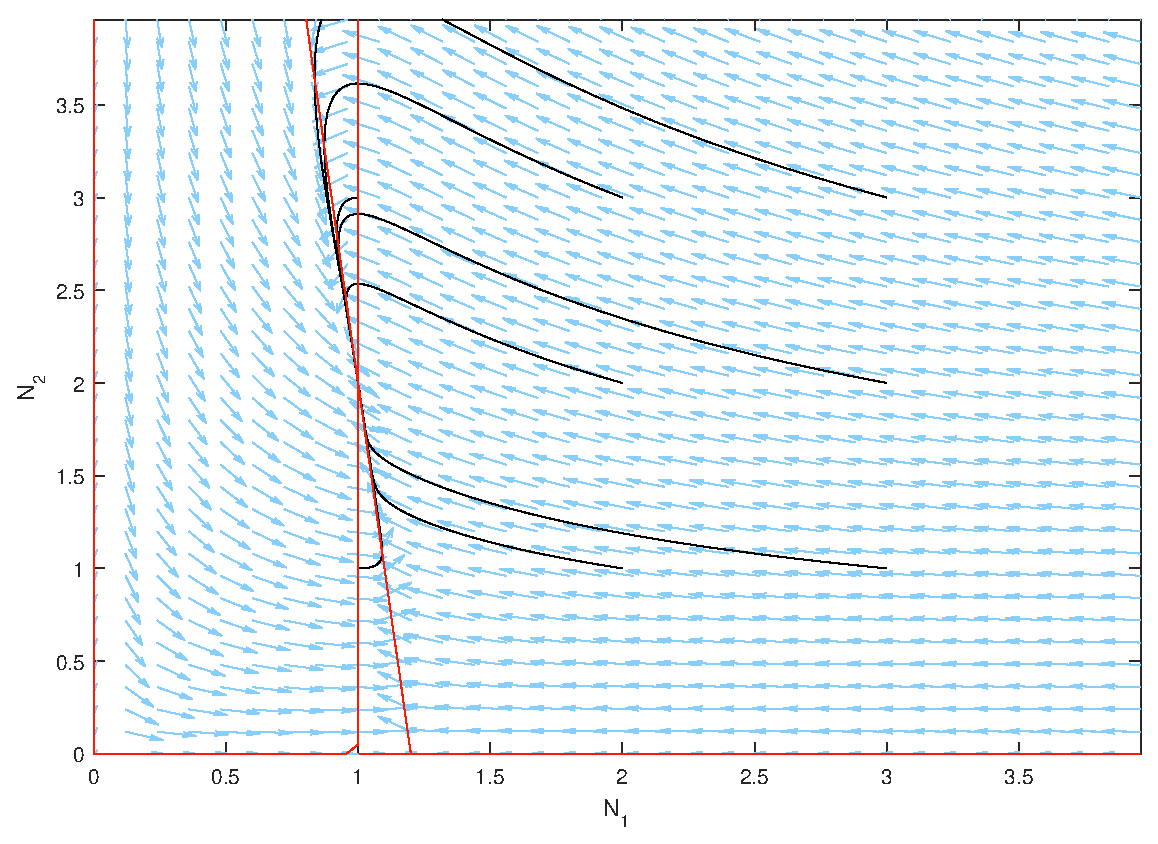
\includegraphics[scale=0.72]{nBeta_StableNode.eps}
	\caption{Predator-prey model with $a=3$, $b=2.5$, $c=0.25$ and $d=e=1$}
	\label{fig3}
\end{figure}

\begin{figure}[h]
	\centering
	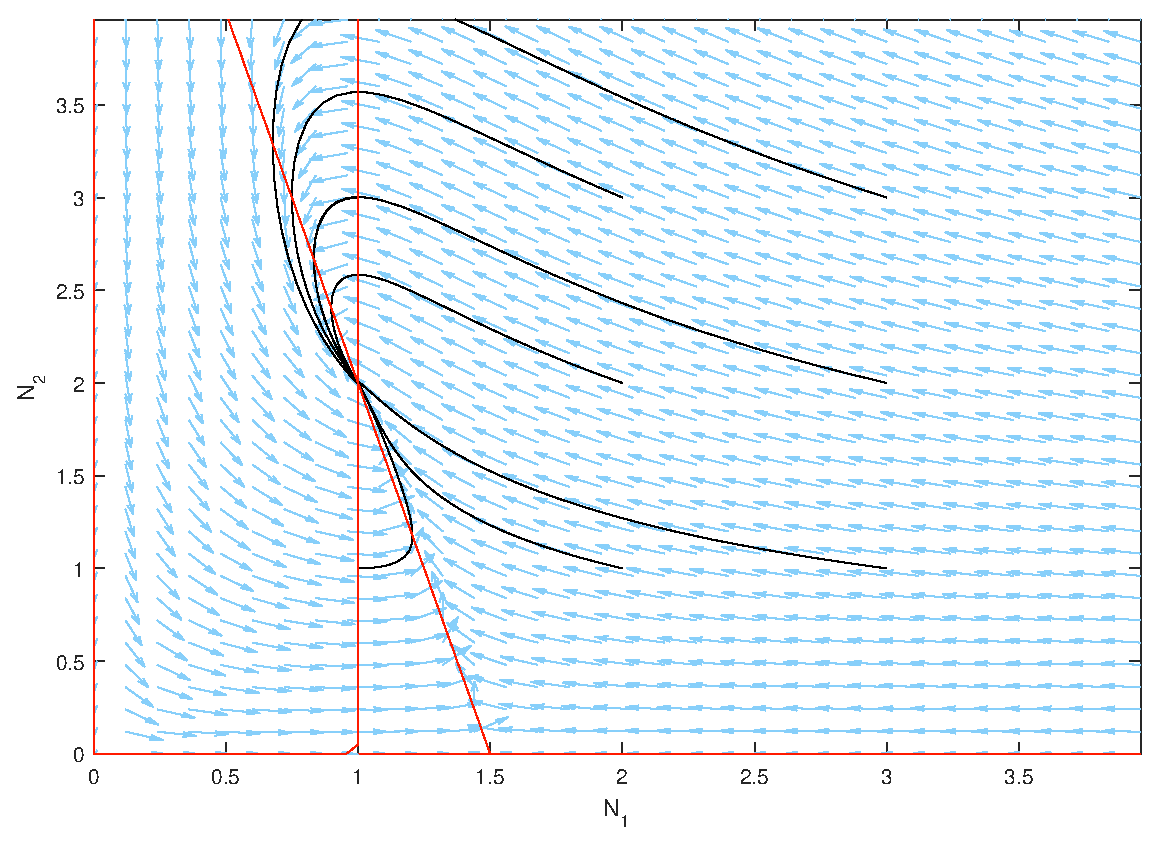
\includegraphics[scale=0.72]{nBeta_MarginalCase.eps}
	\caption{Predator-prey model with $a=3$, $b=2$, $c=0.5$ and $d=e=1$}
	\label{fig4}
\end{figure}

Figure \ref{fig5} corresponds to the case $be=ad$ where $\beta$ and $\gamma$ were classified as non-isolated fixed points in the discussion before. For the chosen coefficients both fixed point collapse in $(1,0)$. Apart from the equilibrium populations and solutions where $N_1 \equiv 0$ all trajectories approach the equilibrium population $(1,0)$ in a convex curve from right to left as $t \rightarrow \infty$. Solutions where $N_1 \equiv 0$ behave as in the cases before. We see that $(1,0)$ is a stable equilibrium population, but it is an isolated fixed point. The basin of attraction around $(1,0)$ is the first quadrant excluding the $N_2$-axis.

\begin{figure}[h]
	\centering
	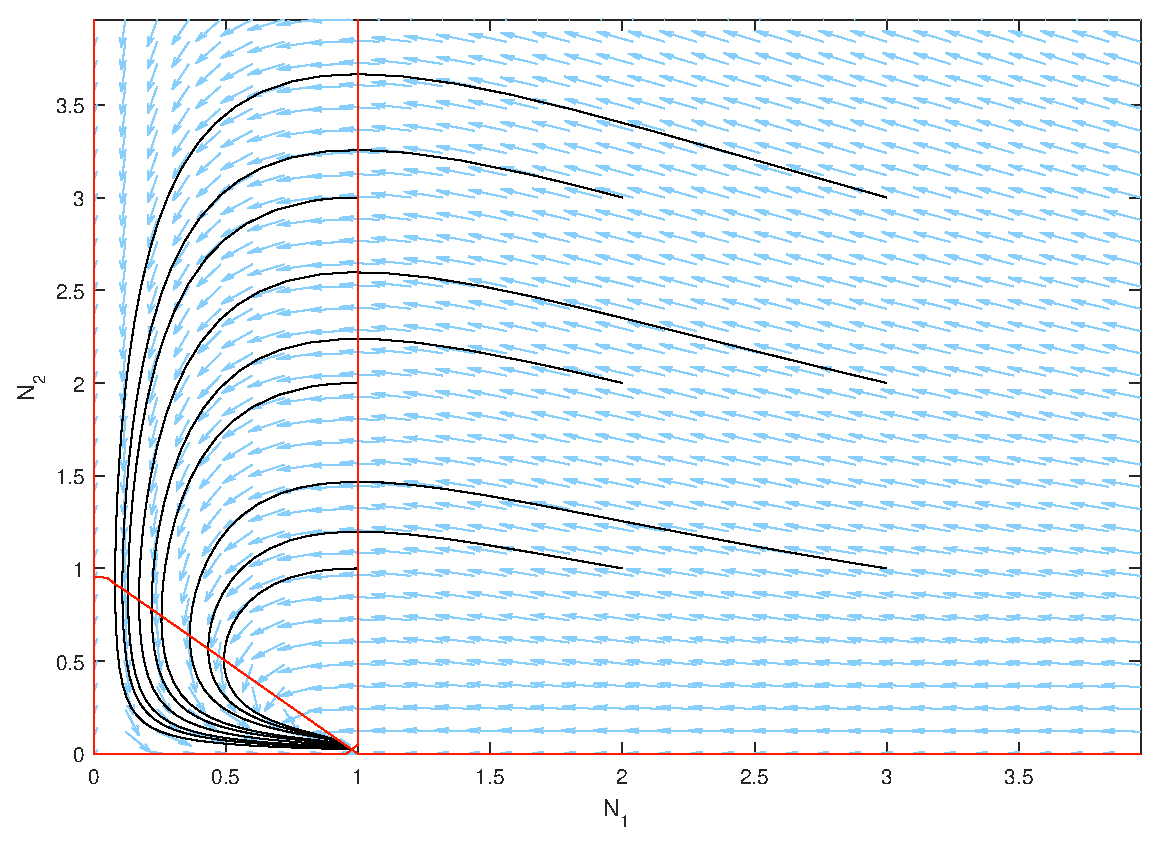
\includegraphics[scale=0.6]{nBeta_NonIsolated.eps}
	\caption{Predator-prey model with $a=b=c=d=e=1$}
	\label{fig5}
\end{figure}

\begin{figure}[h]
	\centering
	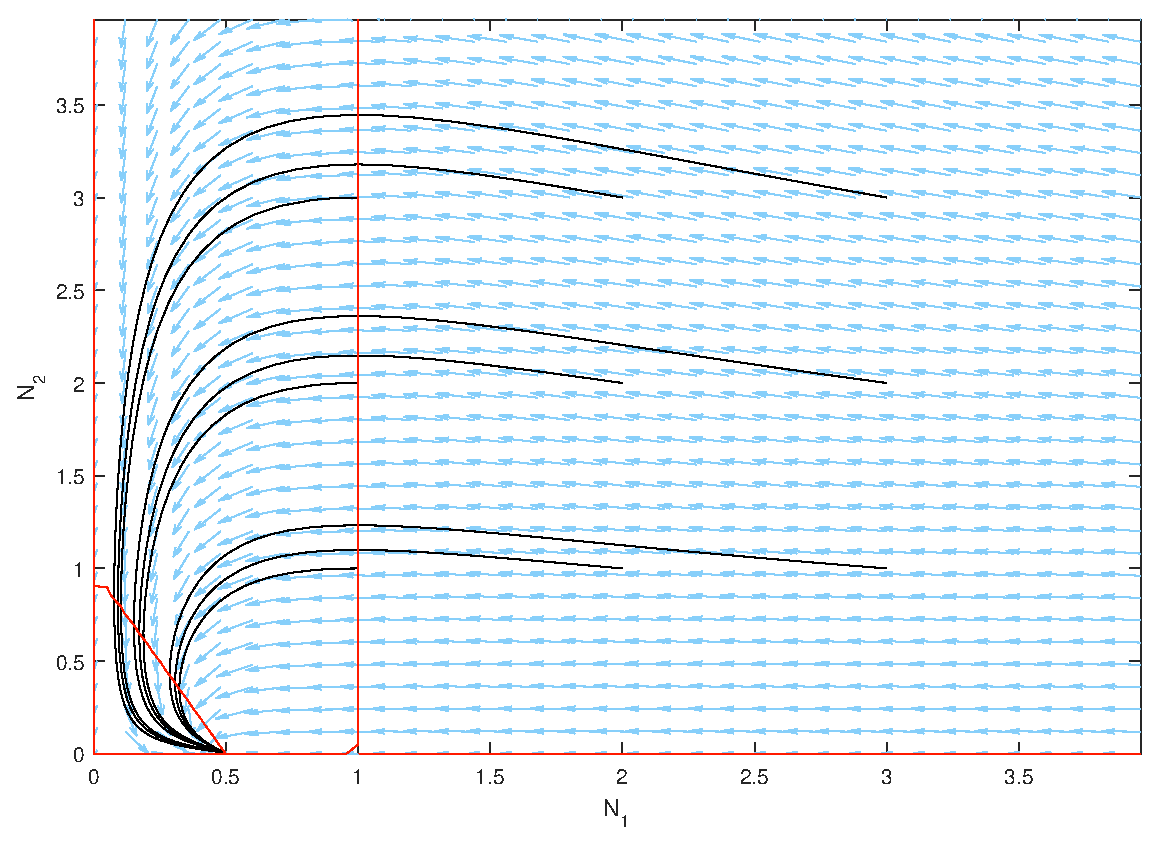
\includegraphics[scale=0.6]{nGamma_StableNode.eps}
	\caption{Predator-prey model with $a=c=d=e=1$ and $b=2$}
	\label{fig6}
\end{figure}

The last case is $be>ad$ where $\beta$ lies outside the first quadrant. Thus, the only interesting equilibrium population in focus is $\gamma$, which is a stable node according to our computations. Figure \ref{fig6} shows this case. We can see that the qualitative behavior of the trajectories in Figure \ref{fig5} and Figure \ref{fig6} are the same. Therefore, the fixed point $(1,0)$ in Figure \ref{fig5} is most likely a stable node, too.
\newline

The careful reader might have noticed that in all examples the equilibrium populations are intersection points of nullclines. This observation holds true in general, because nullclines are zero level sets of the functions $f$ or $g$ as in the definition of equilibrium populations, and thus the intersection points are exactly the points $(N_1,N_2)$ such that $f(N_1,N_2)=0=g(N_1,N_2)$.

\FloatBarrier

\section{Tensorflow Algorithm}

Recall the \textit{logistic equation} for single species we mentioned previously:

\begin{equation} \tag{3}
	\frac{dN}{dt}=N(a-bN). 
\end{equation}

Let us rewrite it as follows:

\begin{equation} \label{eq9}
	\frac{dN}{dt}=rN(1-\frac{N}{K}), 
\end{equation}

where $a=r$ and $b=\frac{r}{K}$. Here, $r$ is the \textit{reproductive rate}, that is to say the number of individuals produced per individual per unit time. $K$ is the \textit{environmental carrying capacity}, that is to say the maximum population size of the species that the environment can carry in the absence of the other species\cite{Murray}. Thus, we get that a system for two species $N_1$ and $N_2$ living in the same environment but not interacting together is:

\begin{equation} \label{eq10}
	\frac{dN_1}{dt}=r_1N_1(1-\frac{N_1}{K_1}),
\end{equation}

\begin{equation} \label{eq11}
	\frac{dN_2}{dt}=r_2N_2(1-\frac{N_2}{K_2}),
\end{equation}

where $r_1$, $r_2$, $K_1$ and $K_2$ $\in \mathbb{R}_{>0}$.
\newline

In the competition model, the two species are interacting with each other. This is called an \textit{interspecific} relationship, because each species has an influence on the growth and the survival of the other. In nature, this happens when two species compete for a same limited resource like food or nesting sites. This situation is detrimental to both species' per capital growth rates $\frac{dN_1}{dt}\frac{1}{N_1}$ and $\frac{dN_2}{dt}\frac{1}{N_2}$ \cite{main}. The competition equations then can be described by the following system of differential equations:

\begin{equation} \label{eq12}
	\frac{dN_1}{dt}=r_1N_1(1-\frac{N_1}{K_1}-b_{12}\frac{N_2}{K_1}),
\end{equation}

\begin{equation} \label{eq13}
	\frac{dN_2}{dt}=r_2N_2(1-\frac{N_2}{K_2}-b_{21}\frac{N_1}{K_2}),
\end{equation}

where $b_{12}$ and $b_{21}$ $\in \mathbb{R}_{>0}$ measure the strength of competitiveness of each species. More precisely, 
$b_{12}$ measures the competitive effect of $N_2$ on $N_1$ and $b_{21}$ measures the competitive effect of $N_1$ on $N_2$.
\newline

In order to ease the next calculations, let us set $x_1=\frac{N_1}{K_1}$, $x_2=\frac{N_2}{K_2}$, $\beta=\frac{r_2}{r_1}$, $\alpha_{12}=b_{12}\frac{K_2}{K_1}$, $\alpha_{21}=b_{21}\frac{K_1}{K_2}$ and a dimensionless time $\tau=r_1t$. We obtain this following new system:

\begin{equation} \label{eq14}
	\frac{dx_1}{d\tau}=x_1(1-x_1-\alpha_{12}x_2)=f_1(x_1, x_2),
\end{equation}

\begin{equation} \label{eq15}
	\frac{dx_2}{d\tau}=\beta x_2(1-x_2-\alpha_{21}x_1)=f_2(x_1, x_2).
\end{equation}

We actually just did what is called a \textit{nondimensionalization}, as we eliminated all the parameters with units. However, it will be important to revert to the original parameters when interpreting the system in ecological terms during the phase plane analysis.

\subsection{Equilibrium Populations and Stability}

The equilibrium populations $(x_1^{*}, x_2^{*}) \in \mathbb{R}^2_{\geqslant 0}$ are solutions of $f_1(x_1, x_2)=f_2(x_1, x_2)=0$. In the competition model, we get four possible equilibrium populations:

\begin{equation*} 
	(x_1^{*}, x_2^{*})\in\Big\{(0,0), (1,0), (0,1), P=(\frac{1-\alpha_{12}}{1-\alpha_{12}\alpha_{21}}, \frac{1-\alpha_{21}}{1-\alpha_{12}\alpha_{21}}) \Big\}.
\end{equation*}

\subsubsection{Existence of the Equilibrium Populations}

Since the populations are non-negative, one should note that the last equilibrium population $P$ only exists if: \Big\{$\alpha_{12} > 1$ and $\alpha_{21} > 1$\Big\}, or \Big\{$\alpha_{12} < 1$ and $\alpha_{21} < 1$\Big\}, or \Big\{$\alpha_{12}=1$ and $\alpha_{21}\neq 1$\Big\}, or \Big\{$\alpha_{21}=1$ and $\alpha_{12} \neq 1$\Big\}.
\newline

Hence, we will have to consider 9 different cases: \Big\{$\alpha_{12} < 1$ and $\alpha_{21} < 1$\Big\}, \Big\{$\alpha_{12} < 1$ and $\alpha_{21} = 1$\Big\}, \Big\{$\alpha_{12} = 1$ and $\alpha_{21} < 1$\Big\}, \Big\{$\alpha_{12} > 1$ and $\alpha_{21} > 1$\Big\}, \Big\{$\alpha_{12} = 1$ and $\alpha_{21} > 1$\Big\}, \Big\{$\alpha_{12} > 1$ and $\alpha_{21} = 1$\Big\}, \Big\{$\alpha_{12} = 1$ and $\alpha_{21} = 1$\Big\}, \Big\{$\alpha_{12} < 1$ and $\alpha_{21} > 1$\Big\}, \Big\{$\alpha_{12} > 1$ and $\alpha_{21} < 1$\Big\}.

\subsubsection{Linearization and Stability}

Again, we want to linearize the system around the equilibrium populations and define the function $F(x_1,x_2)=(f_1(x_1, x_2), f_2(x_1, x_2))$ whose Jacobian matrix is:

\begin{center}
$DF(x_1,x_2)=\begin{pmatrix}
	1-2x_1-\alpha_{12}x_2 & -\alpha_{12}x_1 \\
	- \beta \alpha_{21}x_2 & \beta (1-2x_2-\alpha_{21}x_1)
\end{pmatrix}$.
\end{center}

Let us analyze the stability of each equilibrium:
\newline
\newpage
\underline{Equilibrium $(0, 0)$}

\begin{center}
$\begin{vmatrix}
	DF(0,0)-\lambda I
\end{vmatrix}=\begin{vmatrix}
	1-\lambda & 0 \\
	0 & \beta - \lambda
\end{vmatrix}=(1-\lambda)(\beta-\lambda)=0$ \[ \Rightarrow \left\{ \begin{array}{ll}
         \lambda_1=1 & \mbox{$>0$}\\
        \lambda_2=\beta & \mbox{$>0$} \end{array} \right. \] 
\end{center}

Since the eigenvalues $\lambda$ are positive, $(x_1^{*}, x_2^{*})=(0,0)$ is unstable.

\vspace{1em}
\underline{Equilibrium $(1, 0)$}

\begin{center}
$\begin{vmatrix}
	DF(1,0)-\lambda I
\end{vmatrix}=\begin{vmatrix}
	-1-\lambda & -\alpha_{12} \\
	0 & \beta(1-\alpha_{21}) - \lambda
\end{vmatrix}=(-1-\lambda)(\beta(1-\alpha_{21})-\lambda)=0$ \[ \Rightarrow \left\{ \begin{array}{ll}
         \lambda_1=-1 & \mbox{$<0$}\\
        \lambda_2=\beta(1-\alpha_{21}) \end{array} \right. \] 
\end{center}

We get 3 cases:
\begin{itemize}
\item If $\alpha_{21}<1$, $\lambda_2>0$, so $(x_1^{*}, x_2^{*})=(1, 0)$ is unstable;
\item If $\alpha_{21}=1$, $\lambda_2=0$, so $(x_1^{*}, x_2^{*})=(1, 0)$ is neutrally stable;
\item If $\alpha_{21}>1$, $\lambda_2<0$, so $(x_1^{*}, x_2^{*})=(1, 0)$ is stable.
\end{itemize}

\vspace{1em}
\underline{Equilibrium $(0, 1)$}

\begin{center}
$\begin{vmatrix}
	DF(0,1)-\lambda I
\end{vmatrix}=\begin{vmatrix}
	1-\alpha_{12}-\lambda & 0 \\
	-\beta \alpha_{21} & -\beta - \lambda
\end{vmatrix}=(1-\alpha_{12}-\lambda)(-\beta-\lambda)=0$ \[ \Rightarrow \left\{ \begin{array}{ll}
         \lambda_1=1-\alpha_{12}\\
        \lambda_2=-\beta & \mbox{$<0$} \end{array} \right. \] 
\end{center}

We get 3 cases again:
\begin{itemize}
\item If $\alpha_{12}<1$, $\lambda_1>0$, so $(x_1^{*}, x_2^{*})=(0, 1)$ is unstable;
\item If $\alpha_{12}=1$, $\lambda_1=0$, so $(x_1^{*}, x_2^{*})=(0, 1)$ is neutrally stable;
\item If $\alpha_{12}>1$, $\lambda_1<0$, so $(x_1^{*}, x_2^{*})=(0, 1)$ is stable.
\end{itemize}
\vspace{1em}
\newpage
\underline{Equilibrium $P=(\frac{1-\alpha_{12}}{1-\alpha_{12}\alpha_{21}}, \frac{1-\alpha_{21}}{1-\alpha_{12}\alpha_{21}})$}

\begin{center}
$\begin{vmatrix}
	DF(P)-\lambda I
\end{vmatrix}\vspace{1em}
\newline=\begin{vmatrix}
	1-2\frac{1-\alpha_{12}}{1-\alpha_{12}\alpha_{21}}-\alpha_{12}\frac{1-\alpha_{21}}{1-\alpha_{12}\alpha_{21}}-\lambda & -\alpha_{12}\frac{1-\alpha_{12}}{1-\alpha_{12}\alpha_{21}} \\
	-\beta \alpha_{21}\frac{1-\alpha_{21}}{1-\alpha_{12}\alpha_{21}} & \beta (1-2\frac{1-\alpha_{21}}{1-\alpha_{12}\alpha_{21}} - \alpha_{21}\frac{1-\alpha_{12}}{1-\alpha_{12}\alpha_{21}})-\lambda
\end{vmatrix}\vspace{1em}
\newline=\begin{vmatrix}
	\frac{\alpha_{12}-1}{1-\alpha_{12}\alpha_{21}}-\lambda & \frac{\alpha_{12}(\alpha_{12}-1)}{1-\alpha_{12}\alpha_{21}} \\
	\frac{\beta \alpha_{21}(\alpha_{21}-1)}{1-\alpha_{12}\alpha_{21}} & \frac{\beta(\alpha_{21}-1)}{1-\alpha_{12}\alpha_{21}}-\lambda
\end{vmatrix}=$
$(\frac{\alpha_{12}-1}{1-\alpha_{12}\alpha_{21}}-\lambda)(\frac{\beta(\alpha_{21}-1)}{1-\alpha_{12}\alpha_{21}}-\lambda)-\frac{\beta \alpha_{12}\alpha_{21}(\alpha_{12}-1)(\alpha_{21}-1)}{1-\alpha_{12}\alpha_{21}}=0$ \[ \Rightarrow \] $\beta(\alpha_{12}-1)(\alpha_{21}-1)-\lambda(\alpha_{12}-1)-\lambda \beta (\alpha_{21}-1)+\lambda^2-\beta \alpha_{12}\alpha_{21}(\alpha_{12}-1)(\alpha_{21}-1)=\lambda^2+\lambda(-(\alpha_{12}-1)-\beta(\alpha_{21}-1))+\beta(\alpha_{12}-1)(\alpha_{21}-1)(1-\alpha_{12}\alpha_{21})=0$ \[ \Rightarrow \left\{ \begin{array}{ll}
         \lambda_1=\frac{(\alpha_{12}-1)+\beta(\alpha_{21}-1)+\sqrt{((\alpha_{12}-1)+\beta(\alpha_{21}-1))^2-4\beta(\alpha_{12}-1)(\alpha_{21}-1)(1-\alpha_{12}\alpha_{21})}}{2}\\
        \lambda_2=\frac{(\alpha_{12}-1)-\beta(\alpha_{21}-1)-\sqrt{((\alpha_{12}-1)+\beta(\alpha_{21}-1))^2-4\beta(\alpha_{12}-1)(\alpha_{21}-1)(1-\alpha_{12}\alpha_{21})}}{2} \end{array} \right. \] 
\end{center}

The signs of $\lambda_1$ and $\lambda_2$ depend on $\beta$, $\alpha_{12}$ and $\alpha_{21}$. We cannot easily determine the stability of $P$.

\subsection{Phase Plane Analysis}

In order to plot the phase planes, let us recall that the nullclines are given by:

\begin{equation}\label{eq16}
	f_1(x_1, x_2)=0 \Leftrightarrow 1-x_1-\alpha_{12}x_2=0,
\end{equation}

\begin{equation} \label{eq17}
	f_2(x_1, x_2)=0 \Leftrightarrow 1-x_2-\alpha_{21}x_1=0.
\end{equation}

Let us analyze in more detail some of the nine possible cases mentioned above. A few have been omitted because their phase portraits are symmetrical to those in the cases below.

\subsubsection{Analysis of the Possible Principal Cases}

\underline{Case \Big\{$\alpha_{12} < 1$ and $\alpha_{21} < 1$\Big\}}\newline

\begin{figure}[!ht]
\centering
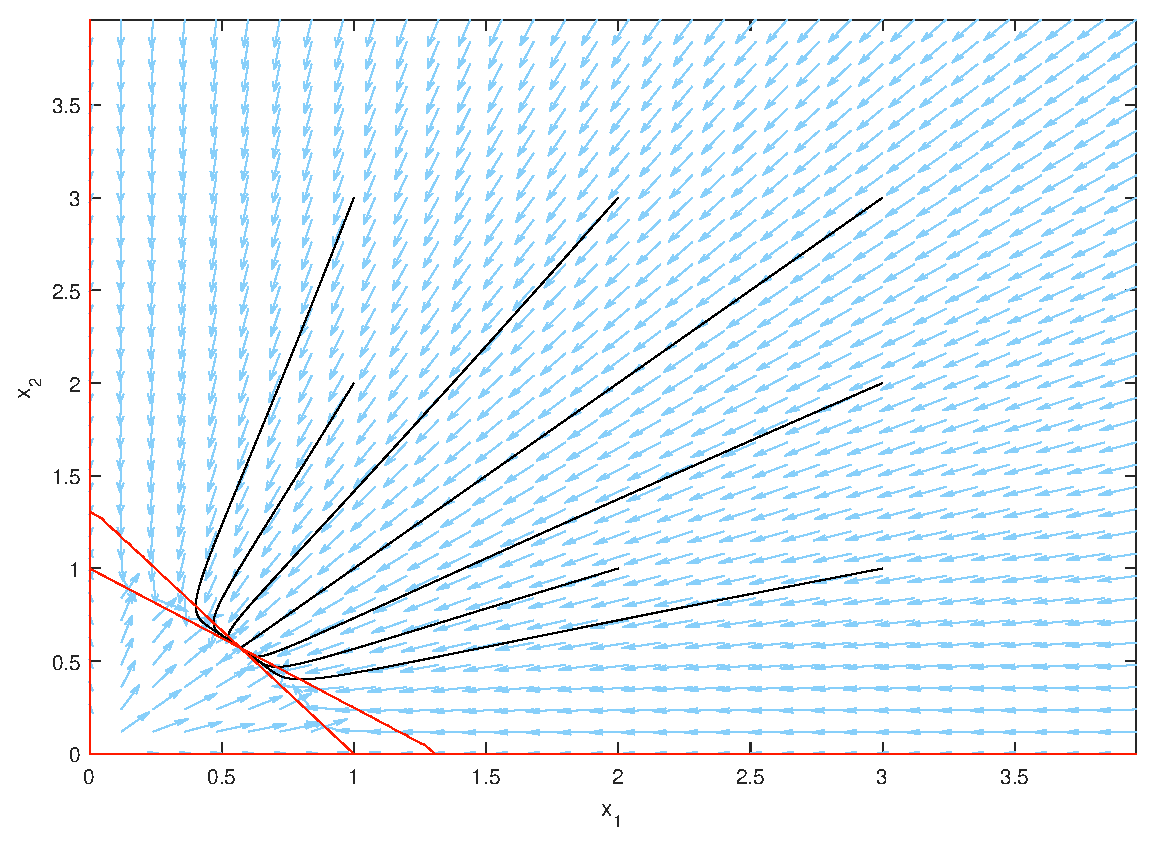
\includegraphics[scale=.6]{fig_1.eps}
\caption{Competition model with $\alpha_{12} < 1$ and $\alpha_{21} < 1$}
\label{figC1}
\end{figure} 

This case has four equilibriums. The equilibriums $(0, 0)$, $(1, 0)$ and $(0, 1)$ are unstable. While $(0, 0)$ is an \textbf{unstable node}, both $(1, 0)$ and $(0, 1)$ are \textbf{saddles}. From the phase portrait, we get that the equilibrium $P$, which here is the intersection of the two non-axes nullclines, attracts all of the interior of $\mathbb{R}_{>0}^2$: it is a \textbf{stable node}. Ecologically, the two species adjust to a lower population size than their respective carrying capacities $K_1$ and $K_2$. This phenomenon is called \textit{coexistence} , as the two species are bad competitors \cite{Murray}.
\FloatBarrier
\vspace{1em}
\underline {Case \Big\{$\alpha_{12} < 1$ and $\alpha_{21} = 1$\Big\}}\newline

\begin{figure}[!ht]
\centering
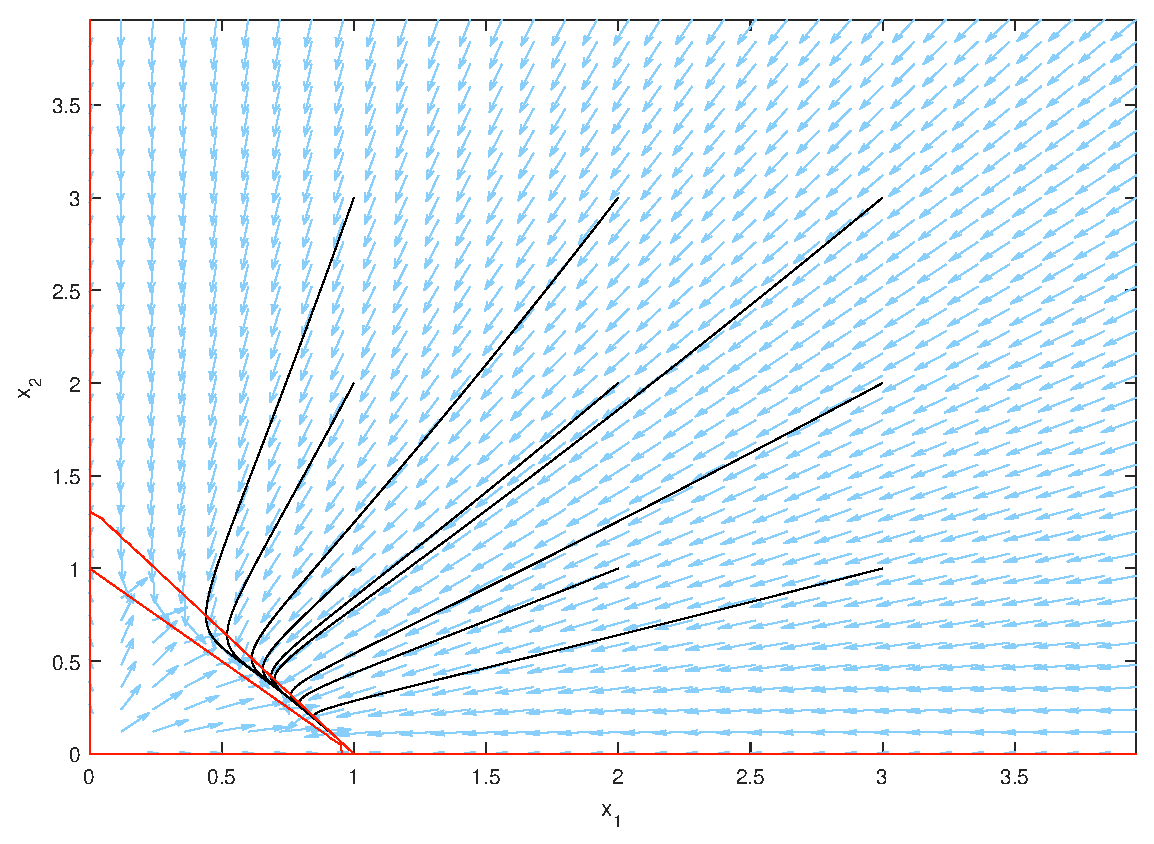
\includegraphics[scale=.6]{fig_2.eps}
\caption{Competition model with $\alpha_{12} < 1$ and $\alpha_{21} = 1$}
\label{figC2}
\end{figure} 

This case has three equilibriums, since we get $P=(1, 0)$. The equilibriums $(0, 0)$ and $(0, 1)$ are unstable, while $(1, 0)$ is neutrally stable. Both $(0, 0)$ and $(0, 1)$ are \textbf{unstable nodes}, while $(1, 0)$ is a \textbf{stable node}. Ecologically, we have that, regardless of the initial conditions, the species $N_2$ is will become extinct while the species $N_1$ tends to its carrying capacity $K_1$. The phase portrait of the case \Big\{$\alpha_{12} = 1$ and $\alpha_{21} < 1$\Big\} is symmetric.
\FloatBarrier
\vspace{1em}
\underline{Case \Big\{$\alpha_{12} > 1$ and $\alpha_{21} > 1$\Big\}}\newline

\begin{figure}[!ht]
\centering
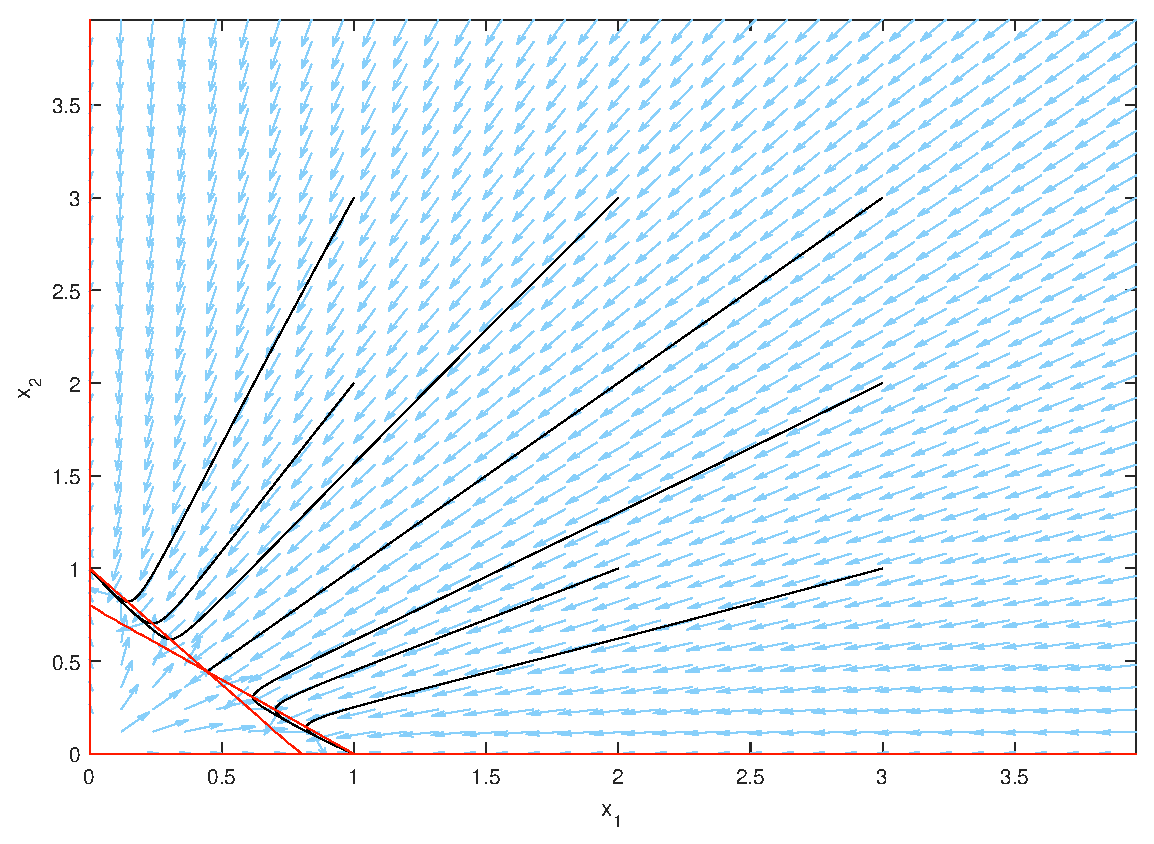
\includegraphics[scale=.6]{fig_4.eps}
\caption{Competition model with $\alpha_{12} > 1$ and $\alpha_{21} > 1$}
\label{figC4}
\end{figure} 

This case is the most interesting one. There are four equilibriums, among which $(1, 0)$ and $(0, 1)$ are stable, while $(0, 0)$ is unstable. Both $(1, 0)$ and $(0, 1)$ are \textbf{stable nodes} and $(0, 0)$ is an \textbf{unstable node}. Furthermore, we get that the eigenvalues of the equilibrium $P$, which are again the intersection of the two non-axes nullclines, are such that $\lambda_2<0<\lambda_1$: so it is unstable and $P$ is a \textbf{saddle}. We see on the phase portrait that the direction of a trajectory to either one of the two stable equilibrium points depends on its position towards the straight line that passes through $P$. This straight line, which splits the phase plane into two non-overlapping regions, is called the \textit{separatrix}. The trajectories converge to $(1, 0)$ above the separatrix and to $(0, 1)$ below it. Trajectories starting on the separatrix and not at the origin, tend to $P$ as the separatrix is indeed one of the saddle trajectories. However, here, it is ecologically impossible to predict which species ultimately wins out, because this result crucially depends on the initial conditions. If initial conditions lie above the separatrix, which means that the species $N_2$ has an initial population size advantage over $N_1$, we get that $x_1$ tends to $0$ and $x_2$ tends to $1$. Thus, the species $N_1$ becomes extinct, while $N_2$ tends to its carrying capacity $K_2$. The exact contrary happens when initial conditions lie under the separatrix. This case implies an inevitable extinction of one species. Even if initial conditions lie on the separatrix, unpredictable random fluctuations will make either one of the species tend to $0$. This case illustrates a phenomenon called \textit{competitive exclusion}. In fact, the two species are competing for the same limited resource and cannot coexist.
\FloatBarrier
\vspace{1em}
\underline{Case \Big\{$\alpha_{12} = 1$ and $\alpha_{21} > 1$\Big\}}\newline

\begin{figure}[!ht]
\centering
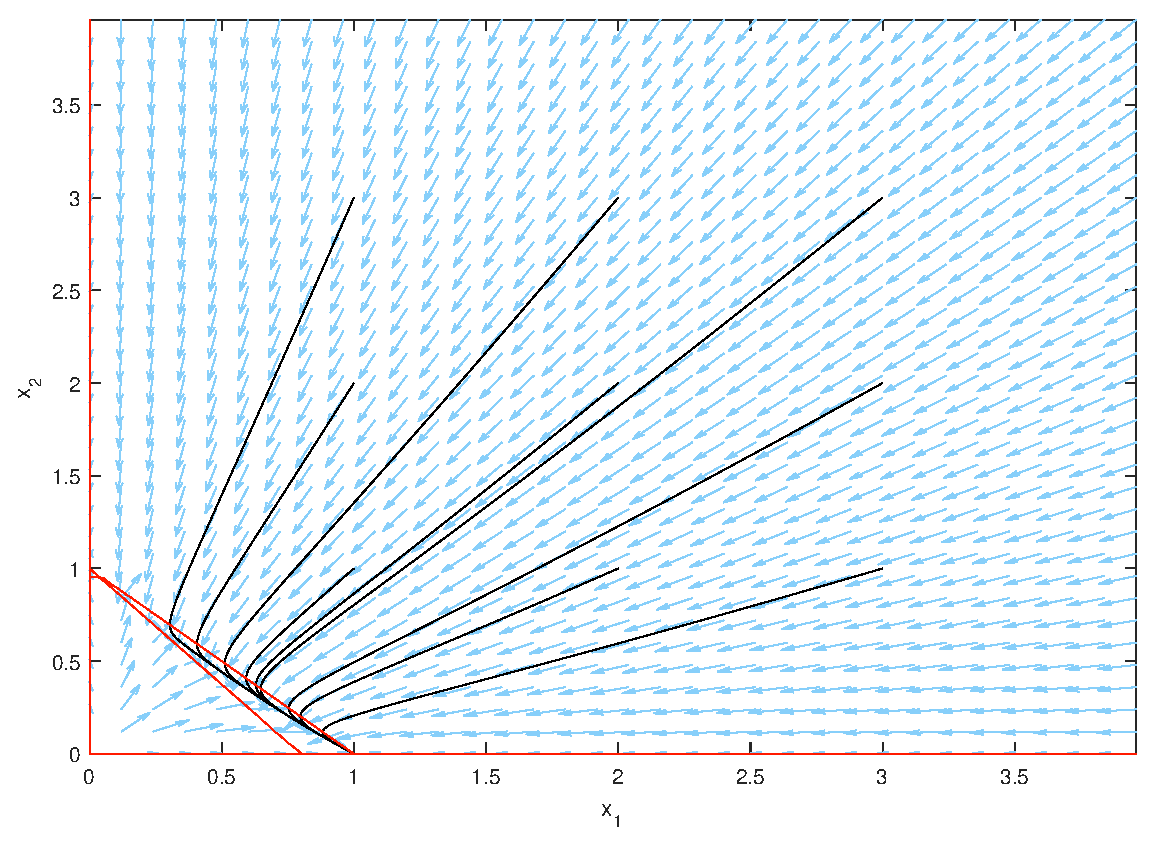
\includegraphics[scale=.6]{fig_5.eps}
\caption{Competition model with $\alpha_{12} = 1$ and $\alpha_{21} > 1$}
\label{figC5}
\end{figure} 

This case has three equilibriums, since we get $P=(0, 1)$. The equilibrium $(0, 0)$ is unstable, $(1, 0)$ is stable and $(0, 1)$ is neutrally stable. The equilibrium $(0, 0)$ is an \textbf{unstable node}, $(1, 0)$ is a \textbf{stable node} and $(0, 1)$ is a \textbf{non-isolated fixed point}. Ecologically, we have that, regardless of the initial conditions, the species $N_2$ will become extinct while the species $N_1$ tends to its carrying capacity $K_1$. This is again a competitive exclusion case \cite{Murray}. The phase portrait of the case \Big\{$\alpha_{12} > 1$ and $\alpha_{21} = 1$\Big\} is symmetric.
\FloatBarrier
\vspace{1em}
\underline{Case \Big\{$\alpha_{12} = 1$ and $\alpha_{21} = 1$\Big\}}\newline

\begin{figure}[!ht]
\centering
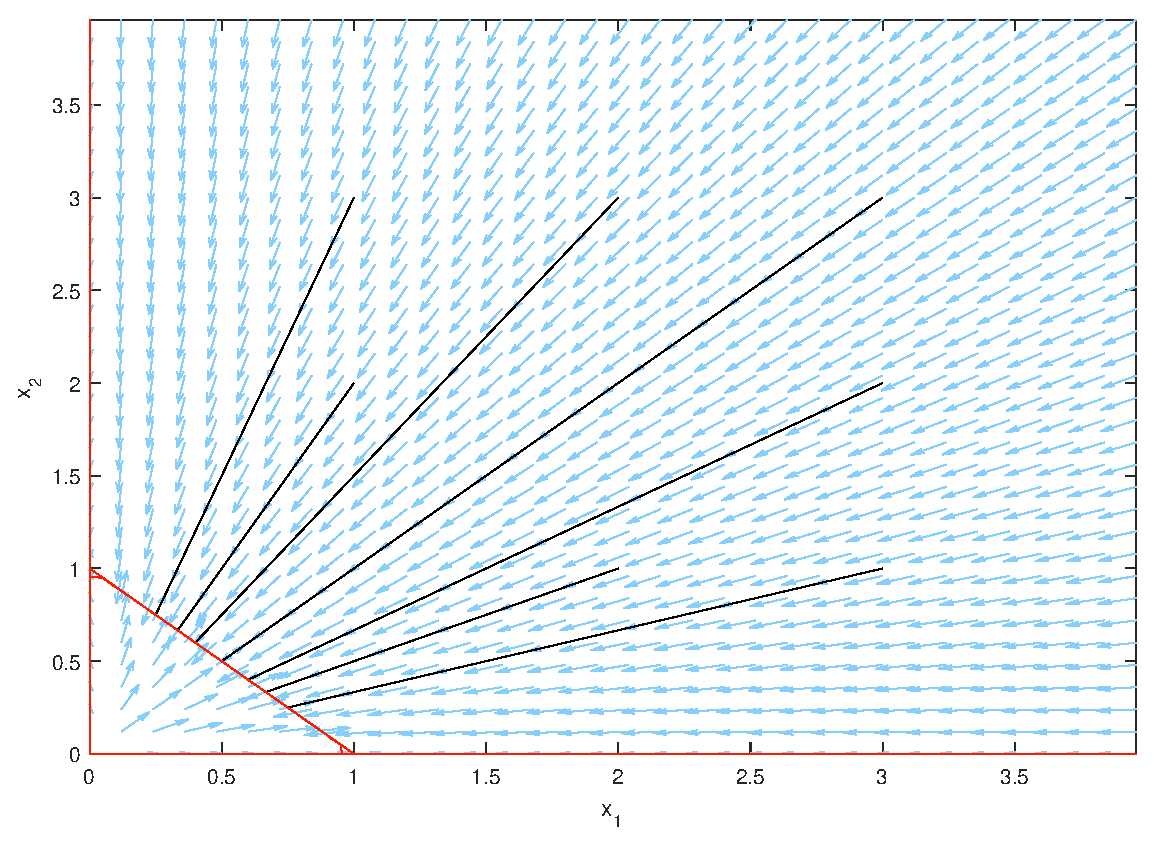
\includegraphics[scale=.6]{fig_7.eps}
\caption{Competition model with $\alpha_{12} = 1$ and $\alpha_{21} = 1$}
\label{figC7}
\end{figure} 

This case is unique in the sense that we have an infinite number of equilibriums. The equilibrium $(0, 0)$ is unstable and it is an \textbf{unstable node}. The two non-axes nullclines are the same and are represented by the single straight line of equation $1-x_1-x_2=0$. As we mentioned it before, Lotka-Volterra intersections of nullclines give all the equilibrium points. But the whole straight line represents an intersection, so we get an infinite number of equilibrium populations on the line between the points $(1, 0)$ and $(0, 1)$. Those equilibriums are neutrally stable. This is a borderline case and, from the phase portrait, we get that those are \textbf{non-isolated fixed points}. The graph indicates that all the trajectories are straight lines. This means ecologically that both population sizes $N_1$, $N_2$ evolve at constant rate and so their ratio is constant until the equilibrium at the straight line is reached.
\FloatBarrier
\vspace{1em}
\underline{Case \Big\{$\alpha_{12} < 1$ and $\alpha_{21} > 1$\Big\}}\newline

\begin{figure}[!ht]
\centering
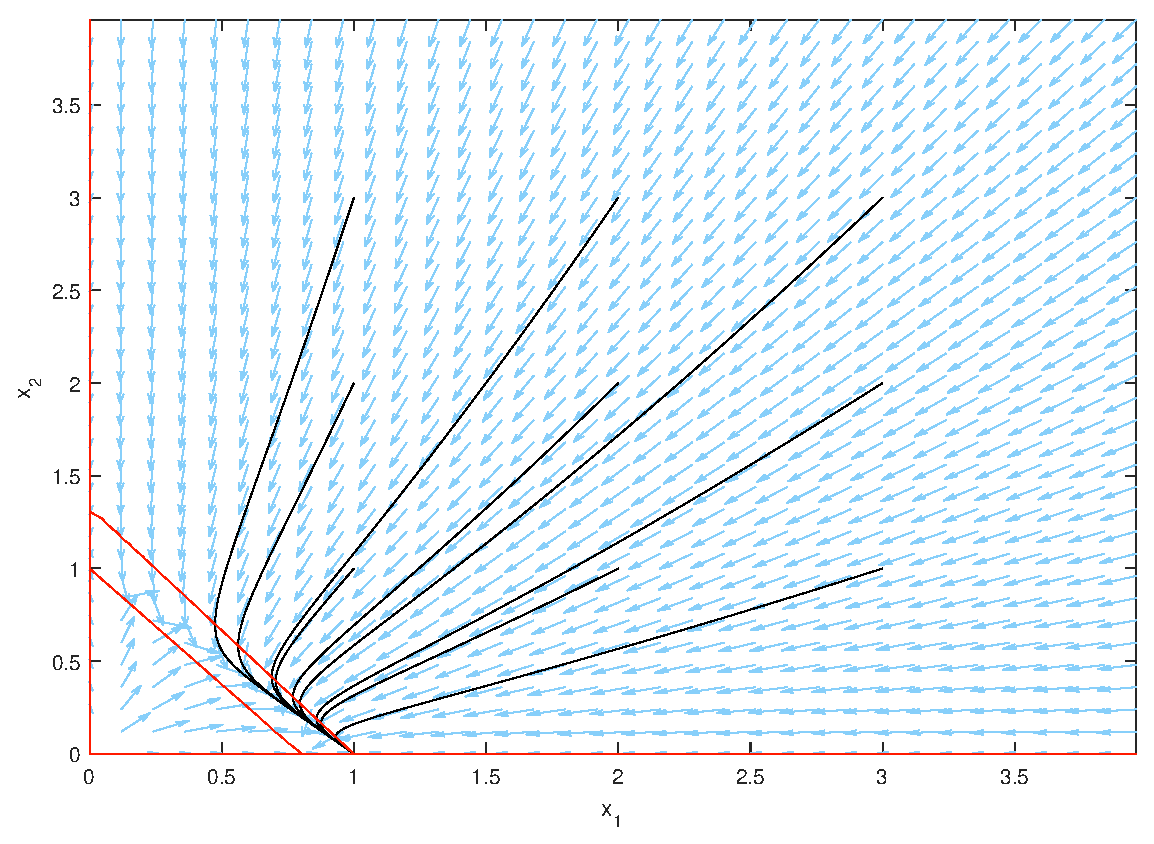
\includegraphics[scale=.6]{fig_8.eps}
\caption{Competition model with $\alpha_{12} < 1$ and $\alpha_{21} > 1$}
\label{figC8}
\end{figure} 

This case has three equilibriums. The equilibrium populations $(0, 0)$ and $(0, 1)$ are unstable, while $(1, 0)$ is stable. While $(1, 0)$ is a \textbf{stable node}, both $(0, 0)$ and $(0, 1)$ are \textbf{unstable nodes}. Ecologically, the species $N_1$ is more aggressive than $N_2$ in obtaining the coveted resources. Regardless of the initial conditions, it is inevitable that $N_1$ dominates and $N_2$ finally becomes extinct. This is again a competitive exclusion case. The phase portrait of the case \Big\{$\alpha_{12} > 1$ and $\alpha_{21} < 1$\Big\} is symmetric.
\FloatBarrier

\subsubsection{General Comments}

Considering all these cases, we see that whatever the parameter values are, the population sizes always tend to a finite equilibrium. There is no population explosion or population oscillations. If one species is a much more aggressive competitor than the other, that species will prevail, tending to its carrying capacity while the other species becomes extinct. If both species are aggressive competitors, then either species may prevail, depending on their respective initial populations. Finally, if either species are bad competitors, then both species coexist, but neither of them reach their respective carrying capacity.


\section{Results}

To begin our discussion of mutualism, let us return to a familiar system of differential equations: 

\begin{equation} \tag{11}
	\frac{dN_1}{dt}=r_1N_1(1-\frac{N_1}{K_1}),
\end{equation}

\begin{equation} \tag{12}
	\frac{dN_2}{dt}=r_2N_2(1-\frac{N_2}{K_2}),
\end{equation}

where $r_1, r_2 \in \mathbb{R}_{>0}$ represent the reproductive rate and $K_1, K_2 \in \mathbb{R}_{>0}$ represent the environmental carrying capacity. $N_1, N_2$ represent the population sizes of generic species living together in an isolated system. So far, our system model only includes a reproduction mechanism and a threshold term $\frac{N_1}{K_1}$. Now, we augment our model with the implication that $N_1$ benefits from the growth of $N_2$ and vise versa, to the extent that the per capital growth rates increase linearly with the population size of the other species. We will henceforth refer to this new system of differential equations as the "mutualism equations" which are described below:

\begin{equation} \label{eq18}
	\frac{dN_1}{dt}=r_1N_1(1-\frac{N_1}{K_1}+b_{12}\frac{N_2}{K_1}),
\end{equation}

\begin{equation} \label{eq19}
	\frac{dN_2}{dt}=r_2N_2(1-\frac{N_2}{K_2}+b_{21}\frac{N_1}{K_2}),
\end{equation}

with $b_{12}, b_{21} \in \mathbb{R}_{>0}$ reflecting the advantage the species' obtain from one another.

Unlike the Competition Model, there are no ecological restrictions that prevent $b_{12}$ and $b_{21}$ from being equal. Furthermore, in our Mutualism Model, we must attend to the fact that no species negatively affects the other; rather, the environment is the only restraining factor in this model. Thus, our qualitative focus is binary: either the advantage gained from interspecific interaction exceeds the threshold term or it does not. The former implying that the population will blow up, causing our model to fall short of any applied mathematical reasoning, and the latter implying that our population will converge to a equilibrium population positioned at the center of the first quadrant, created by a mutual maximum population threshold.
\newline

\subsection{Equilibrium Populations}

For the sake of simplicity, let us set $K_1$ and $K_2$ to be 1. Furthermore, let us set $r_1$ and $r_2$ to be 2. Thus, our above system becomes:

\begin{equation} \label{eq20}
	\frac{dN_1}{dt}=2N_1(1-N_1+b_{12}N_2)=f_1(N_1, N_2),
\end{equation}

\begin{equation} \label{eq21}
	\frac{dN_2}{dt}=2N_2(1-N_2+b_{21}N_1)=f_2(N_1, N_2).
\end{equation}

The equilibrium populations $(x_1^{*}, x_2^{*}) \in \mathbb{R}^2_{\geqslant 0}$ are solutions of $f_1(N_1, N_2)=f_2(N_1, N_2)=0$. In the mutualism model, we get four possible equilibrium populations:

\begin{center}
	$(x_1^{*}, x_2^{*}) \in \Big\{(0,0), (1,0), (0,1), (\frac{1+b_{12}}{1-b_{12}b_{21}}, \frac{1+b_{21}}{1-b_{12}b_{21}})\Big\}$.
\end{center}

We are particularly interested in the last equilibrium population $(x_1^{*}, x_2^{*})=(\frac{1+b_{12}}{1-b_{12}b_{21}}, \frac{1+b_{21}}{1-b_{12}b_{21}})$ which will dictate the said centralized first quadrant equilibrium population.\newline

Note again that the terms equilibrium population and fixed point are synonymous.

\subsubsection{Linearization of the System}

Let us define a vector $F(N_1,N_2)=(f_1(N_1, N_2), f_2(N_1, N_2))$. The corresponding Jacobian matrix is: 

\begin{center}
$DF(N_1,N_2)=\begin{pmatrix}
	2-4N_1+2b_{12}N_2 & 2b_{12}N_1 \\
	2b_{21}N_2 & {2-4N_2+2b_{21}N_1}
\end{pmatrix}_{(N_1,N_2)}$
\end{center}

We will utilize this linearized matrix to classify the fixed points in the following section. To assist in the linearization and classification process, we have written a simple \textit{GNU Octave} function called\textit{ linearize\_classify(f, g, x1, y1)} which accepts two scalar functions $f$, $g$ and a fixed point $(x1,y1)$. The function displays the Jacobian matrix, eigenvalues, and the classification of the fixed point. The source code for the function is available at the end of the Discussion section. 

\subsection{Stability and Phase Plane Analysis}

We will organize our parameter case studies around the values of $b_{12}$ and $b_{21}$. Before the analysis begins, the reader should note that modeling mutualism as a separate module is not optimal in some cases. One key weakness of the Lotka-Volterra inspired mutulism equations is that they fail to model relationships where mutualism is critical to the birthing mechanism of a species. For example, Heijden and Horton found that 48\% of land plants rely on mycorrhizal relationships (mutualistic relationship between a fungus and the roots of a land plant) for survival \cite{Van}. Nonetheless, our rudimentary analysis will offer the reader a succinct comprehension of the Mutualism Model. The source code to produce these phase portraits is available at the end of the Discussion section.
\newline\newline
\underline{Case 1: $b_{12} = 0.3$ and $b_{21} = 0.4$}
\newline\newline
Equations \eqref{eq20} and \eqref{eq21} now become 

\begin{equation} \label{eq22}
	\frac{dN_1}{dt}=2N_1(1-N_1+0.3N_2)=f_1(N_1, N_2),
\end{equation}

\begin{equation} \label{eq23}
	\frac{dN_2}{dt}=2N_2(1-N_2+0.4N_1)=f_2(N_1, N_2).
\end{equation}

\begin{figure}[!ht]
\centering
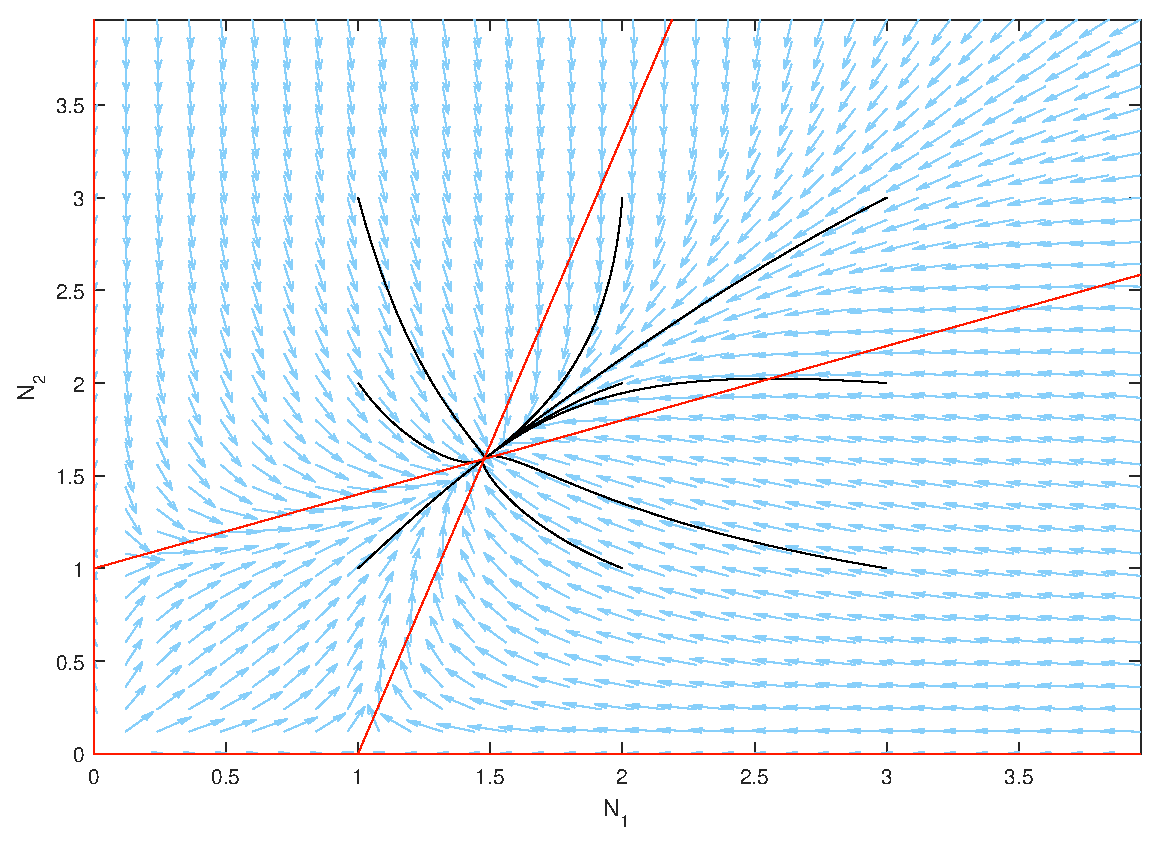
\includegraphics[scale=.72]{fig1.eps}
\centering
\caption{Mutualism model with  $b_{12} = 0.3$ and $b_{21} = 0.4$}
\label{figM1}
\end{figure}

 Let us utilize \textit{linearize\_classify} to evaluate fixed points $(x_1^{*}, x_2^{*}) \in \Big\{(0,0), (1,0), (0,1), (\frac{65}{44}, \frac{35}{22}) \Big\}$. The following display omits the Jacobian matrix and eigenvalues.
\newline
>> syms x y\newline
>> f = 2*x-2*x*x+0.6*y*x;\newline
>> g = 2*y-2*y*y+0.8*x*y;\newline
>> linearize\_classify (f, g, 0, 0)\newline
\textbf{The fixed point is a degenerate node.}\newline
\textbf{Warning: This is a borderline case; we can not make any qualitative assumptions about the nonlinear system.}\newline
>> linearize\_classify (f, g, 0, 1)\newline
\textbf{The fixed point is a saddle point.}\newline
>> linearize\_classify (f, g, 1, 0)\newline
\textbf{The fixed point is a saddle point.}\newline
>> linearize\_classify (f, g, $\frac{65}{44}, \frac{35}{22}$)\newline
\textbf{The fixed point is an stable node.}\newline

\begin{definition}{\textbf{\textit{Stable Manifold}}}
\newline
In reference to a saddle point $x^*$, a stable manifold is defined as the set of initial conditions $x_0$ such that $x(t) \rightarrow x^{*}$ as $
t \rightarrow \infty$ \cite{main}.
\end{definition}

As we can see the from Figure \ref{figM1}, each and every fixed point besides the borderline case at (0,0) is accurate. One thing to note about the fixed points (0,1) and (1,0): the stable manifolds are represented by the y and x axis respectively.\newline

Case 1 warrants special consideration in the basin of attraction discussion. The fortunate confinement of two stable manifolds causes the entire first quadrant to become a basin of attraction!\newline

There are four nullclines in this case: $N_1$=0, $N_2$=0,  $N_2=\frac{10}{3}N_1-\frac{10}{3}$, and  $N_2=\frac{2}{5}N_1+1$. \textit{The nullclines $N_1$=0, $N_2$=0 are present in every case}. The intersection of the red nullclines $N_2=\frac{10}{3}N_1-\frac{10}{3}$ and $N_2=\frac{2}{5}N_1+1$ produces a central fixed point $(\frac{65}{44},\frac{35}{22})$ where the mutual maximum population threshold occurs; all first quadrant trajectories converge to this stable node fixed point as $t \rightarrow \infty$. Case 1 demonstrates how mutualism would work in a typical biological environment: no matter how successful the species' are at helping each other, they will always be restrained by their environmental limitations. Ultimately, $b_{12}$ and $b_{21}$ were too low to surpass the threshold term.\newline

\underline{Case 2: $b_{12} = 1$ and $b_{21} = 2$}
\newline\newline
Equations \eqref{eq20} and \eqref{eq21} now become 

\begin{equation} \label{eq24}
	\frac{dN_1}{dt}=2N_1(1-N_1+N_2)=f_1(N_1, N_2),
\end{equation}

\begin{equation} \label{eq25}
	\frac{dN_2}{dt}=2N_2(1-N_2+2N_1)=f_2(N_1, N_2).
\end{equation}

\begin{figure}[!ht]
\centering
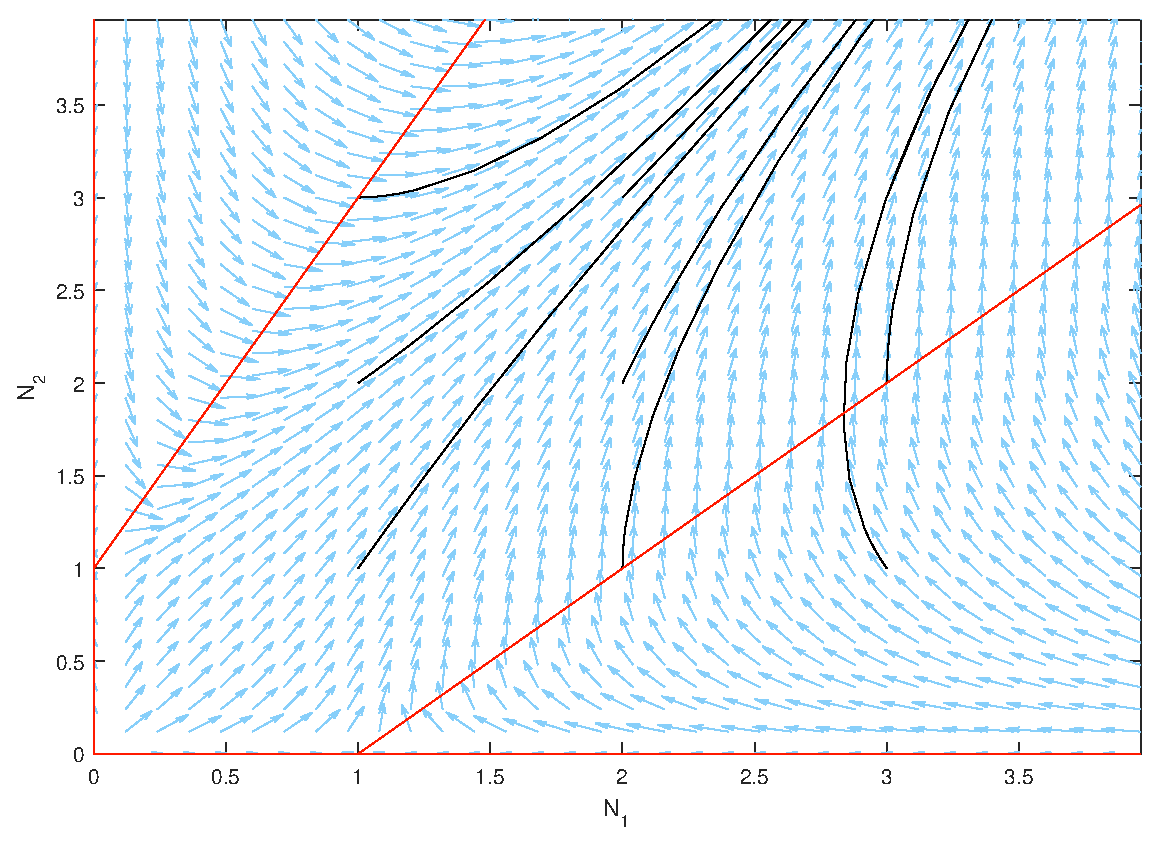
\includegraphics[scale=.72]{fig3.eps}
\caption{Mutualism model with $b_{12} = 1$ and $b_{21} = 2$}
\label{figM2}
\end{figure}

Let us again evaluate the fixed points $(x_1^{*}, x_2^{*}) \in \Big\{(0,0), (1,0), (0,1), (-2,-3) \Big\}$ with \newline\textit{linearize\_classify}, omitting the Jacobian matrix and eigenvalues.
\newline
>> syms x y\newline
>> f = 2*x-2*x*x+2*y*x;\newline
>> g = 2*y-2*y*y+4*x*y;\newline
>> linearize\_classify (f, g, 0, 0)\newline
\textbf{The fixed point is a degenerate node.}\newline
\textbf{Warning: This is a borderline case; we can not make any qualitative assumptions about the nonlinear system.}\newline
>> linearize\_classify (f, g, 0, 1)\newline
\textbf{The fixed point is a saddle node.}\newline
>> linearize\_classify (f, g, 1, 0)\newline
\textbf{The fixed point is a saddle point.}\newline
>> linearize\_classify (f, g, -2, -3)\newline
\textbf{The fixed point is a saddle point.}\newline

Figure \ref{figM2} demonstrates the population blow up. Notice that the increase in the values of $b_{12}$ and $b_{21}$ caused the nullclines $N_2=N_1-1$ and $N_2=2N_1+1$ to intersect in the third quadrant and produce a saddle point at (-2,-3). The trajectories never end up converging in the first quadrant. This is the qualitative case in which the population blows up and surpasses the environmental constraints. $b_{12}$ and $b_{21}$ are large enough to surpass the threshold term, causing $N_1,N_2$ increase to infinity as $t \rightarrow \infty$.\newline\newline
The two possible qualitative cases that occur in the Mutualism Model have been presented to the reader. However, there is one salient question left to investigate. When does this system produce a saddle point in third quadrant, a stable node in the first quadrant, or neither case? More specifically, what relationship between $b_{21}$ and $b_{12}$ produces said qualitative expressions in the phase portrait?
\newline\newline
\underline{Case 3: $b_{12} = 1.111$ and $b_{21} = 1$}
\newline\newline
Equations \eqref{eq20} and \eqref{eq21} now become 

\begin{equation} \label{eq26}
	\frac{dN_1}{dt}=2N_1(1-N_1+1.111N_2)=f_1(N_1, N_2),
\end{equation}

\begin{equation} \label{eq27}
	\frac{dN_2}{dt}=2N_2(1-N_2+1N_1)=f_2(N_1, N_2).
\end{equation}

Case 3 gives us a clue. We see in Figure \ref{figM3} that the nullclines are almost parallel but there is still a saddle point in the third quadrant. If instead $b_{12}$ = 1, then the nullclines would be parallel and there would be no intersection: neither a saddle node in the third quadrantn or stable node in the first quadrant occurs! Finally, if $b_{12}$ = 1 - $\epsilon$ where $\epsilon$ is some number slightly larger than 0, we can conjecture that a stable node would emerge in the first quadrant. \newline

To definitely answer the looming question, we must return to beginning.
Setting the $\frac{dN_1}{dt}$ and $\frac{dN_2}{dt}$ in \eqref{eq18} \eqref{eq19} equal to 0:
$\begin{cases} r_1N_1(1-\frac{N_1}{K_1}+b_{12}\frac{N_2}{K_1})=0 \\ r_2N_2(1-\frac{N_2}{K_2}+b_{21}\frac{N_1}{K_2})=0 \end{cases}\vspace{1em} \Rightarrow \begin{cases}1-\frac{N_1}{K_1}+b_{12}\frac{N_2}{K_1}=0 \\ 1-\frac{N_2}{K_2}+b_{21}\frac{N_1}{K_2}=0 \end{cases} \Rightarrow \begin{cases}b_{12}\frac{N_2}{K_1}=\frac{N_1}{K_1}-1 \\ \frac{N_2}{K_2}=b_{21}\frac{N_1}{K_2}+1 \end{cases} \Rightarrow \begin{cases} N_2=\frac{N_1}{b_{12}}-\frac{K_1}{b_{12}} \\ N_2=b_{21}N_1+K_2 \end{cases}$\newline\newline

To produce parallel nullclines, the two equations above must have the same slope. \textbf{The borderline case is therefore when $b_{21}=\frac{1}{b_{12}}$, regardless of what $K_1,K_2,r_1,r_2$ are!} As it turns out, simplifying the model by setting $K_1,K_2$ and $r_1,r_2$ to equal respective values in $\mathbb{R}_{\geqslant 0}$ was completely unnecessary. Working from the parallel borderline slope case, increasing either $b_{21}$ or $b_{12}$ will produce an saddle node intersection in the third quadrant and the inequality $b_{21}>\frac{1}{b_{12}}$, corresponding with population blow up. Alternatively, decreasing either $b_{21}$ or $b_{12}$ will create a stable node intersection in the first quadrant and the inequality $b_{21}<\frac{1}{b_{12}}$, corresponding with a practical mutual maximum population threshold. Let us test this assertion on Case 1 and Case 2: \newline\newline 0.4 < $\frac{1}{0.3}$ meaning in Case 1 the trajectories converge to a central stable node in the first quadrant \checkmark \newline 2 > $\frac{1}{1}$ meaning in Case 2 the population blows up \checkmark
\begin{figure}[!ht]
\centering
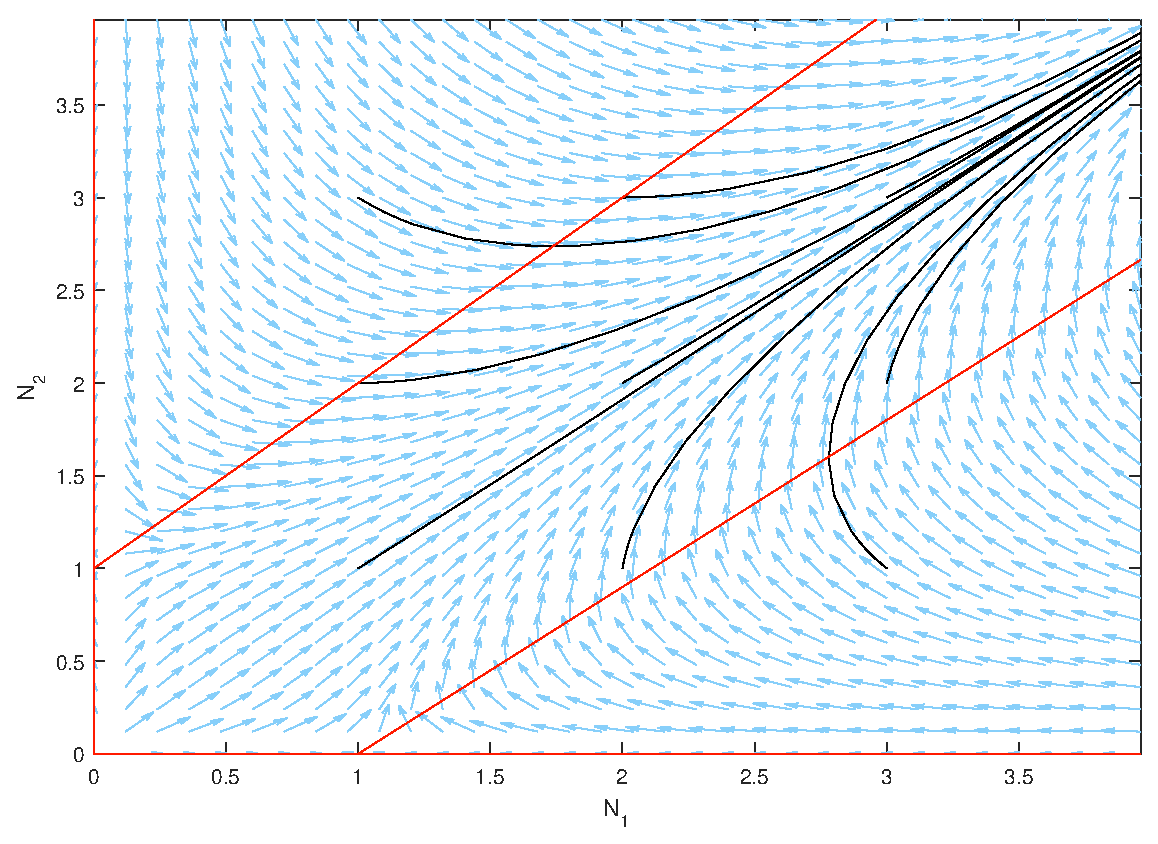
\includegraphics[scale=.72]{fig4.eps}
\caption{Near borderline case}
\label{figM3}
\end{figure}

\section{Discussion}
\lstset{showstringspaces=false}
Although the Lotka-Volterra equations used in this paper are by far the most popular in the mathematics community, there are some alternate equation models worth noting.\newline

The Nicholson-Bailey equations were also developed in the early $20^{th}$ century and are used to model parasite-host systems but can be adapted for predator-prey models \cite{Logan}. The model equations are purely discrete:

\begin{equation} \label{eq28}
	H_{t+1}=\beta H_te^{-\alpha P_t}
\end{equation}

\begin{equation} \label{eq29}
	P_{t+1}=\gamma H_t(1-e^{-\alpha P_t})
\end{equation}

The population sizes of the host and parasite are represented by H and P respectively. $\beta \in \mathbb{R}_{>0}$ is the rate at which the host reproduces, $\alpha\in \mathbb{R}_{>0}$ is the rate at which the parasite disseminates, and $\gamma \in \mathbb{R}_{>0}$ is the rate at which the parasite reproduces in the host. Immediately, we can see that the parasite inflicts exponential population decay on the host. The rate at which the host population decays depends entirely on $\alpha$. Perhaps a Lotka-Volterra system could model certain macro-parasites, that is, parasites visible to the naked eye as they would behave much like a large prey eating predator would. However, a Lotka-Volterra system could never truly capture the reproduction rate of a micro-parasite on the scale of bacteria and viruses.\newline

On the other hand, the Arditi-Ginzburg equations directly compete with the Lotka-Volterra equations. Instead of a growth/decay rate which is a function of population size, Arditi-Ginzburg created a model which relies on the ratio of predator to prey:

\begin{equation} \label{eq30}
	\frac{dN}{dt}=f(N)N-g(\frac{N}{P})P
\end{equation}

\begin{equation} \label{eq31}
	\frac{dP}{dt}=\epsilon g(\frac{N}{P})P-\kappa P
\end{equation}

The function f(N) represents the reproduction rate and $\epsilon$ is a constant which measures the relationship between prey consumption and reproduction. The function g(N/P) represents the effect predators have on the per capita prey population. The Arditi-Ginzburg model is subject to intense debate in the mathematical biology field. Some laud its ability to capture the concept of prey consumption drop off with the increase of predator density. Others deem it an over-complication of the subject matter \cite{ratio1}.
\subsection{Programs}
The following two programs are referenced throughout this paper and are defined below.
\subsubsection{linearize\_classify.m}
\lstinputlisting[language=Octave]{linearize_classify.m}
\textit{linearize\_classify} utilizes the eigenvalue method of fixed point classification. It takes the Jacobian matrix of each input function and then makes a composite $2x2$ Jacobian matrix. Then the eigenvalues are extracted out and parsed. If one of the two eigenvalues has an imaginary component, then we look at the real portion of that eigenvalue: positive implies unstable spiral, $0$ implies a center in which case a energy conservation study must be conducted, and negative implies stable spiral. If one of the two eigenvalues does not have an imaginary component then we compare the signs of the real portions: opposite signs imply a saddle point, two negative signs imply a stable node, two positive signs imply a unstable node; however, if both eigenvalues are equal, then it is a borderline case and we cannot assume anything about the nonlinear system. Furthermore, if one of the eigenvalues is $0$, then we are faced with another borderline case in which case, nothing can be gleaned from our linearization.\newline
\subsubsection{phaseP.m}
\lstinputlisting[language=MATLAB]{phaseP.m}
\textit{phaseP} illustrates the vector field, nullclines and trajectories of a two-dimensional system of differential equations. It evaluates the given function handles $l$ and $k$ at a grid depending on the vector $S$. The vector $(l(x,y), k(x,y))$ correspond to the tangent vector of a solution trajectory at a point $(x,y)$ of the grid. The different tangent vectors are then normalized by their length, and plotted by the built-in function \textit{quiver}. The predefined function \textit{ode45} computes solution trajectories $z(t)=(x(t),y(t))$ satisfying the initial condition $z(0)=(a,b)$. These trajectories are added to the vector field. The built-in function \textit{ezplot} is used to plot the zero level curves of $l$ and $k$, which are by definition the nullclines of the system.
\vspace{1em}


\begin{thebibliography}{7}
\bibitem{Murray} Murray, James Dickson. 
\emph{Mathematical Biology I. an Introduction}, $3^{rd}$ Edition.
N.p.: Springer Verlag, 2014. N. pag. Print.

\bibitem{Haberman} Haberman, Richard. \emph{Mathematical Models: Mechanical Vibrations, Population Dynamics, and Traffic Flow: And Introduction to Applied Mathematics.} Philadelphia: Society for Industrial and Applied Mathematics, 2006. 225-27. Print.

\bibitem{Van} Van Der Heijden, Marcel G. A., and Thomas R. Heijden. "Socialism in Soil? The Importance of Mycorrhizal Fungal Networks for Facilitation in Natural Ecosystems." \emph{Journal of Ecology} 97.6 (2009): 1139-150. Print.

\bibitem{Logan} Logan, J. David; Wolesensky, Willian R. (2009). \emph{Mathematical Methods in Biology}. Pure and Applied Mathematics: a Wiley-interscience Series of Texts, Monographs, and Tracts. John Wiley \& Sons. p. 214. ISBN 978-0-470-52587-6.

\bibitem{ratio} "Coupling in predator-prey dynamics: Ratio-Dependence" (PDF). \emph{ac.els-cdn.com}. Retrieved 2015-09-28.

\bibitem{ratio1}"The nature of predation: prey dependent, ratio dependent or neither?". \emph{Trends in Ecology}. 15: 337–341. doi:10.1016/S0169-5347(00)01908-X. Retrieved 2015-09-28.

\bibitem{main} Strogatz, Steven H. \emph{Nonlinear Dynamics and Chaos: With Applications to Physics, Biology, Chemistry, and Engineering}. 2nd ed. Boulder, CO: Westview, a Membeer of the Perseus Group, 2015. Print.
\end{thebibliography}
\end{document}